%!TEX root = ../dokumentation.tex

\chapter{Einleitung}

Schach ist ein Strategiespiel, dessen Wurzeln im 6. Jahrhundert in Indien liegen. In den letzten Jahren erlebt das Spiel einen bemerkenswerten Aufschwung, 
welcher vor allem auf die Entwicklung von Online-Plattformen und Events zurückzuführen ist. 
Das Spiel wird auf einem Brett mit 64 Feldern gespielt. Es teilt sich auf in acht Reihen welche nummeriert werden und acht Spalten, die von \(a\) bis \(h\) deklariert werden. 
Die Felder wechseln dabei immer abwechselnd die Farbe. Jeder Spieler beginnt das Spiel mit 16 Figuren: Einem König, einer Dame, zwei Türmen, zwei Springern, zwei Läufern und acht Bauern.
Das Spiel ist zu Ende, sobald ein Spieler keinen legalen Spielzug mehr hat, oder 50 Züge ohne einen Bauern- oder Schlagzug gespielt werden. 

Das Internet hat Spielern die Möglichkeit gegeben sich weltweit gegeneinander zu messen. Online-Plattformen helfen den Spielern mit Funktionen wie Spielanalysen und Rätseln besser zu werden.
In 2022 erreichte die Onlineplattform Chess.com eine Nutzerzahl von über 100.000.000 Spielern. 

\begin{figure}[h]
    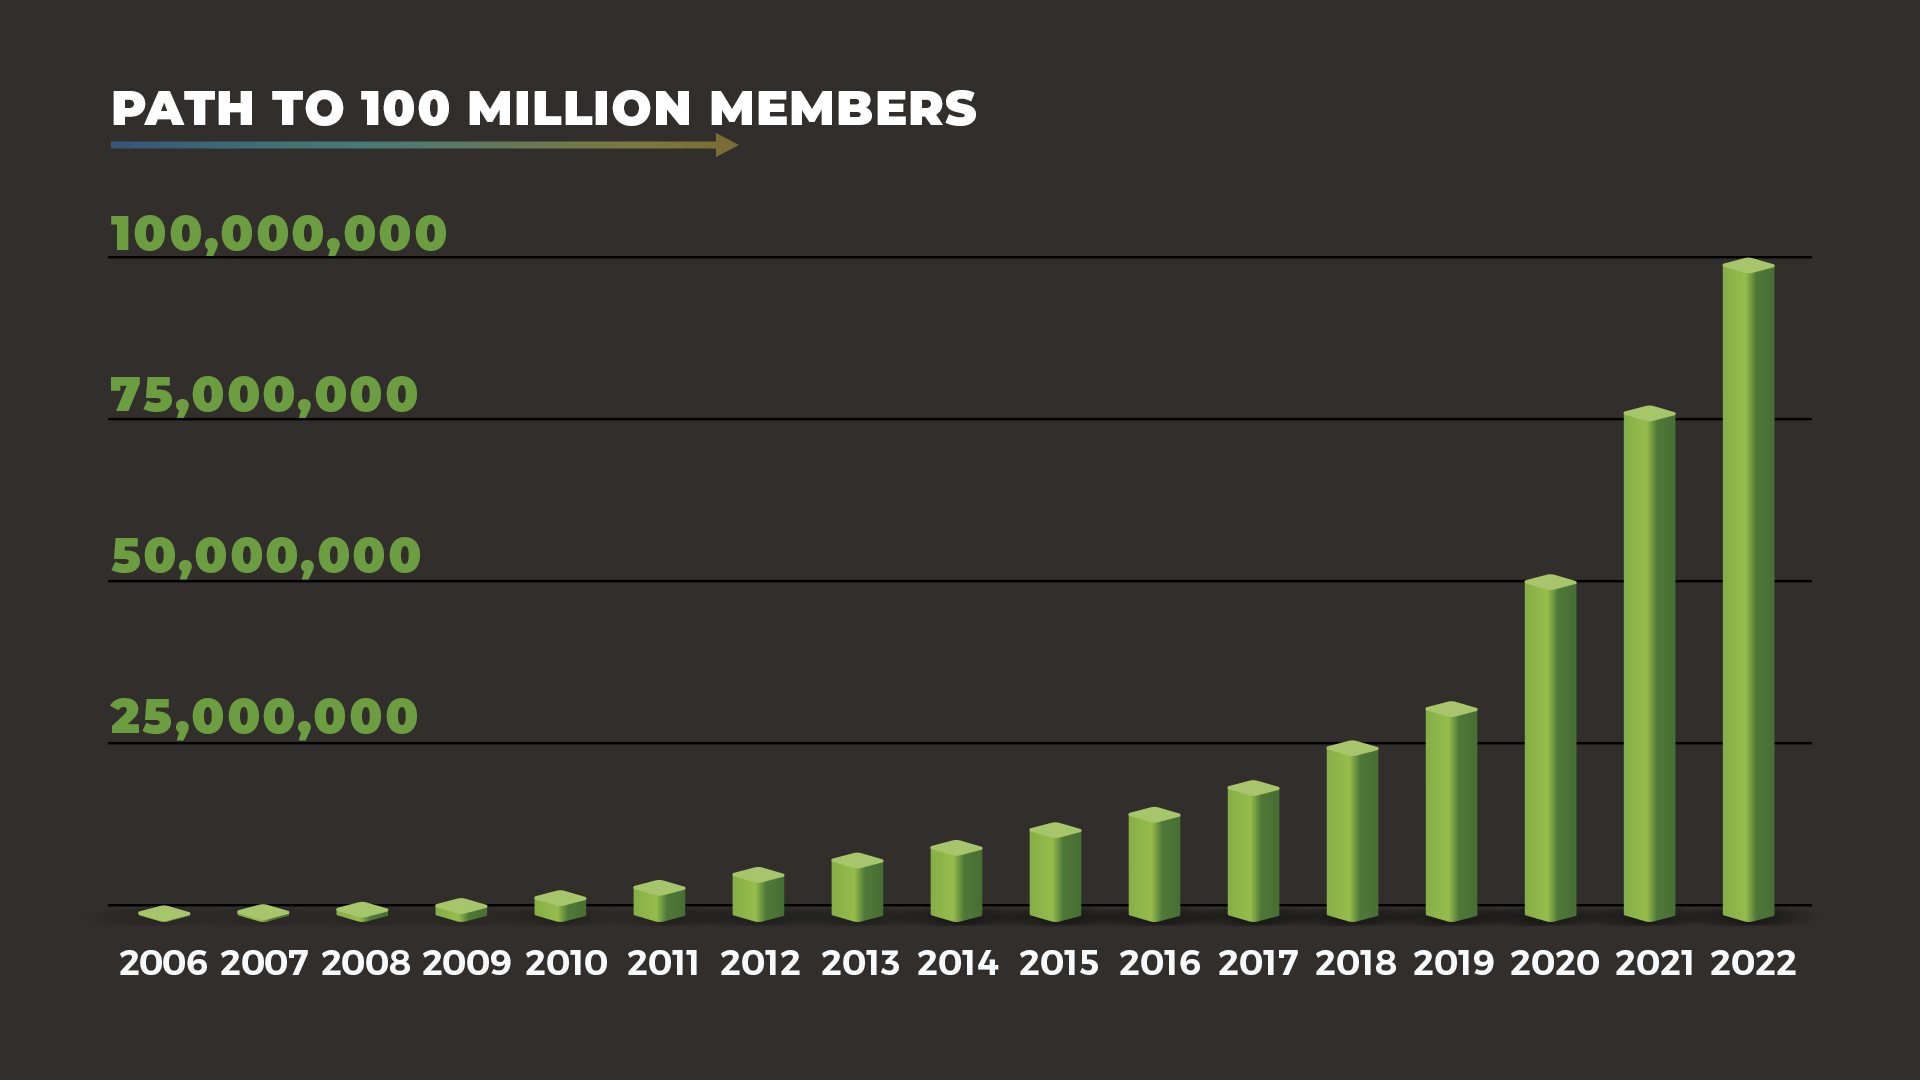
\includegraphics[scale=0.2]{images/chess.com_users.png}
    \caption{Chess.com Spielerzahlen Stand 2022}
\end{figure}

Darüber hinaus hat das Aufkommen von Live-Streaming-Plattformen wie Twitch die Art und Weise, wie Schach als Zuschauer konsumiert wird revolutioniert. 
Bekannte Spieler aus der Szene, aber auch Streamer aus anderen Sektoren zeigen hier ihre Spiele und veranstalten Turniere. 
Weitere Faktoren für den aktuellen Erfolg des Spiels ist die Netflix Serie Queens Gambit aus dem Jahr 2020, die den Weg eines Mädchens zu einer 
Profispielerin zeigt, sowie der Lockdown im selben Jahr.

\section{Motivation}
Durch die zunehmende Begeisterung für das Spielen am Computer rückt das Spiel am Brett immer mehr in den Hintergrund. 
Eine Möglichkeit die Vorteile des online Schachs und die des Brettspiels zu kombinieren ist ein DGT Smart Board. Es wird über Bluetooth 
oder USB mit dem Computer verbunden und ermöglicht dem Spieler die Züge auf einem Brett zu spielen. 
Anschließend werden die Züge an den Computer übertragen. Diese speziellen Bretter sind durch ihren hohen Preis jedoch nicht sehr attraktiv für die meisten Spieler. 
Die Idee dieser Smartboards legt die Grundlage dieses Projektes aus, welches eine Kombination aus einem realen Schachbrett und dem Computer bildet.

\section{Zielsetzung dieser Arbeit}
Ziel dieser Arbeit ist es eine Python Applikation zu entwickeln, mit welcher der Nutzer gegen einen Computer Schach spielen kann. 
Dabei soll es dem Spieler möglich sein, seine Züge auf einem realen Schachbrett zu spielen. Die gespielten Züge werden dann 
mithilfe einer Kamera an die Applikation übertragen. Somit kann Kostengünstig das Erlebnis des Online Schachs mit dem Gefühl des 
Brettspiels kombiniert werden.

Für die Implementierung der Regeln des Spiels werden keine bestehenden Bibliotheken benutzt. Der Schachcomputer soll entweder selber entwickelt werden,
oder es soll ein bestehender Computer genutzt werden.

\pagebreak
\section{Forschungsschwerpunkte}
Um die Zielsetzung zu erreichen, soll diese Arbeit folgende Aspekte behandeln:

\begin{enumerate}
    \item Digitale Bildverarbeitung
    \item Algorithmen für Schachcomputer
    \item Objektorientierte Programmierung in Python
\end{enumerate}
 
\section{Struktur}
Kapitel 2 befasst sich mit den Feinheiten der digitalen Bildverarbeitung, einem wichtigen technologischen Aspekt, 
der bei der Entwicklung des Schachsystems genutzt wurde. Dieser Abschnitt umfasst Unterpunkte zu Bildgrundlagen, Vorverarbeitung, Farbfilterung, 
Formerkennung, Segmentierung, Transformation und Merkmalsextraktion.

Danach kommt eine Einführung in die Grundlagen der Architektur und Funktionalität von Schachcomputern.
Es wird aufgezeigt welche Algorithmen in diesen Computern verwendet werden und welche verschiedenen Ansätze es gibt.
Vor allem wird zwischen Computern mit und ohne maschinellen Lernen unterschieden.

Kapitel 4 diskutiert Überlegungen zur Benutzeroberfläche und zur Programmiersprache. Hier wird die Wahl der Programmiersprache gerechtfertigt, 
in der Entwicklung verwendete Bibliotheken werden aufgezeigt und das Design von Benutzeroberflächen sowie Überlegungen zur Benutzererfahrung werden untersucht. 

Im Anschluss wird die Erstellung der Anwendung erklärt. Das Design und die Architektur des Systems werden erläutert und der Spielverlauf sowie 
die Herausforderungen während des Entwicklungsprozesses werden aufgezeigt.

Das letzte Kapitel enthält das Fazit und die zukünftigen Aussichten. Hier werden die wichtigsten Ergebnisse aus der Arbeit 
zusammengefasst und ein Ausblick auf potenzielle zukünftige Arbeiten und Verbesserungen gegeben.